\documentclass[a4paper]{report}

% --- Paquetes ---------------------------------------------------------------
\usepackage[utf8]{inputenc}
\usepackage[a4paper,
            left=3cm, right=2.5cm,
            top=2.5cm, bottom=2.5cm]{geometry}
\usepackage{setspace}
\usepackage{fancyhdr}
\usepackage{graphicx}
\usepackage[hidelinks]{hyperref}
\usepackage{listings}
\usepackage{xcolor}
\usepackage{array}
\usepackage{tabularx}
\usepackage{booktabs}
\usepackage{longtable}
\usepackage{float}
\usepackage{url}
\usepackage{tocloft}
\usepackage{titlesec}
\usepackage{tikz}
\usepackage{amsmath}
\usepackage{enumitem}
\usepackage{microtype}
\usepackage{parskip}

% --- Fuente sans-serif (Arial equivalente) ----------------------------------
\usepackage[spanish,activeacute,es-tabla,es-noquoting]{babel}
\usepackage{helvet}
\renewcommand{\familydefault}{\sfdefault}

% --- Interlineado 1,5 -------------------------------------------------------
\onehalfspacing

% --- Colores ----------------------------------------------------------------
\definecolor{darkblue}{RGB}{0,51,102}
\definecolor{lightblue}{RGB}{173,207,230}
\definecolor{codegreen}{rgb}{0,0.55,0}
\definecolor{codegray}{rgb}{0.5,0.5,0.5}
\definecolor{codepurple}{rgb}{0.45,0,0.75}
\definecolor{backcolour}{rgb}{0.96,0.96,0.96}
\definecolor{codered}{rgb}{0.75,0,0}

% --- Cabeceras y pies --------------------------------------------------------
\pagestyle{fancy}
\fancyhf{}
\fancyhead[L]{\small\leftmark}
\fancyhead[R]{\small FPConnect -- Manual de Usuario}
\fancyfoot[C]{\thepage}
\renewcommand{\headrulewidth}{0.4pt}
\setlength{\headheight}{14pt}

% --- Hipervínculos -----------------------------------------------------------
\hypersetup{
  colorlinks=true,
  linkcolor=darkblue,
  citecolor=darkblue,
  urlcolor=darkblue
}

% --- Formato de títulos ------------------------------------------------------
\titleformat{\chapter}[display]
  {\normalfont\LARGE\bfseries\color{darkblue}}
  {\chaptertitlename\ \thechapter}{16pt}{\Huge}
\titlespacing*{\chapter}{0pt}{20pt}{30pt}

\titleformat{\section}
  {\normalfont\Large\bfseries\color{darkblue}}{\thesection}{1em}{}
\titlespacing*{\section}{0pt}{16pt}{8pt}

\titleformat{\subsection}
  {\normalfont\large\bfseries\color{darkblue}}{\thesubsection}{1em}{}
\titlespacing*{\subsection}{0pt}{12pt}{6pt}

% ════════════════════════════════════════════════════════════════════════════
\begin{document}
% ════════════════════════════════════════════════════════════════════════════

% --- PORTADA ----------------------------------------------------------------
\begin{titlepage}
  \thispagestyle{empty}
  \centering
  
  % Logo del centro
  \vspace*{0.5cm}
  
\includegraphics[width=5cm]{images/logo.png}
  
  \vspace*{1.5cm}

  {\fontsize{36}{42}\selectfont\bfseries\color{darkblue} FPCONNECT \par}

  \vspace{0.6cm}
  {\fontsize{20}{24}\selectfont\bfseries Manual de Usuario \par}

  \vspace{1cm}
  \textcolor{darkblue}{\rule{12cm}{1pt}}
  \vspace{0.8cm}

  {\fontsize{13}{16}\selectfont\itshape
  Guía completa de uso de la plataforma social para\\[4pt]
  estudiantes de Formación Profesional, centros educativos y empresas \par}

  \vfill

  {\fontsize{12}{15}\selectfont
  \begin{tabular}{rl}
    \textbf{Centro:}          & CES Lope de Vega \\[6pt]
    \textbf{Proyecto:}        & Trabajo Final de Grado (TFG) \\[6pt]
    \textbf{Ciclo:}           & Desarrollo de Aplicaciones Multiplataforma (DAM) \\[6pt]
    \textbf{Versión:}         & 1.0 \\[6pt]
    \textbf{Fecha:}           & \today \\
  \end{tabular}
  \par}

  \vspace{2cm}
  \textcolor{darkblue}{\rule{12cm}{1pt}}
\end{titlepage}

% --- ÍNDICE -----------------------------------------------------------------
\pagestyle{fancy}
\tableofcontents
\newpage

% ════════════════════════════════════════════════════════════════════════════
\chapter*{Introducción}
\addcontentsline{toc}{chapter}{Introducción}
% ════════════════════════════════════════════════════════════════════════════

Bienvenido a \textbf{FPConnect}, la red social profesional especializada para el sector de la Formación Profesional en Andalucía. Este manual te guiará a través de todas las funcionalidades y características disponibles en la plataforma, independientemente de tu rol de usuario (Alumno, Centro Educativo o Empresa).

FPConnect ha sido diseñada para facilitar la conexión entre alumnos, centros educativos y empresas, creando un ecosistema digital donde puedas:

\begin{itemize}
  \item Construir tu red profesional y conectar con otros compañeros del sector
  \item Buscar y gestionar oportunidades de empleo y prácticas (FCT)
  \item Compartir experiencias, consejos y conocimientos del sector
  \item Recibir notificaciones sobre noticias relevantes de Formación Profesional
  \item Comunicarte en tiempo real con otros usuarios
\end{itemize}

Esta guía está organizada por secciones según tu tipo de usuario. Selecciona la que corresponda a tu perfil para obtener instrucciones detalladas.

\newpage

% ════════════════════════════════════════════════════════════════════════════
\chapter{Acceso y Registro}
% ════════════════════════════════════════════════════════════════════════════

\section{Crear una nueva cuenta}

El registro en FPConnect es rápido y gratuito. Sigue estos pasos:

\begin{enumerate}
  \item Accede a la página principal de FPConnect en tu navegador web
  \item Haz clic en el botón \textbf{``Registrarse''} en la esquina superior derecha
  \item Completa el formulario con los siguientes datos:
  \begin{itemize}
    \item \textbf{Email:} Tu dirección de correo electrónico (será tu usuario)
    \item \textbf{Contraseña:} Una contraseña segura (mínimo 8 caracteres, con mayúsculas y números)
    \item \textbf{Nombre:} Tu nombre completo
    \item \textbf{Perfil:} Selecciona tu tipo de usuario:
    \begin{itemize}
      \item \textbf{Soy Alumno:} Si eres estudiante de Formación Profesional
      \item \textbf{Soy Centro FP:} Si representas a un centro educativo
      \item \textbf{Soy Empresa:} Si eres empresa o responsable de RRHH
    \end{itemize}
  \end{itemize}
  \item Haz clic en \textbf{``Registrarse''} para confirmar
  \item ¡Ya estás dentro! Tu cuenta se ha creado correctamente
\end{enumerate}

\section{Iniciar sesión}

Si ya tienes una cuenta en FPConnect:

\begin{enumerate}
  \item En la página principal, haz clic en \textbf{``Iniciar Sesión''}
  \item Introduce tu email y contraseña
  \item Puedes optar por:
  \begin{itemize}
    \item Iniciar sesión con tu email y contraseña
    \item Usar la opción \textbf{``Continuar con Google''} si tu email está vinculado a una cuenta de Google
  \end{itemize}
  \item Haz clic en \textbf{``Iniciar Sesión''} para acceder
\end{enumerate}

\begin{figure}[H]
  \centering
  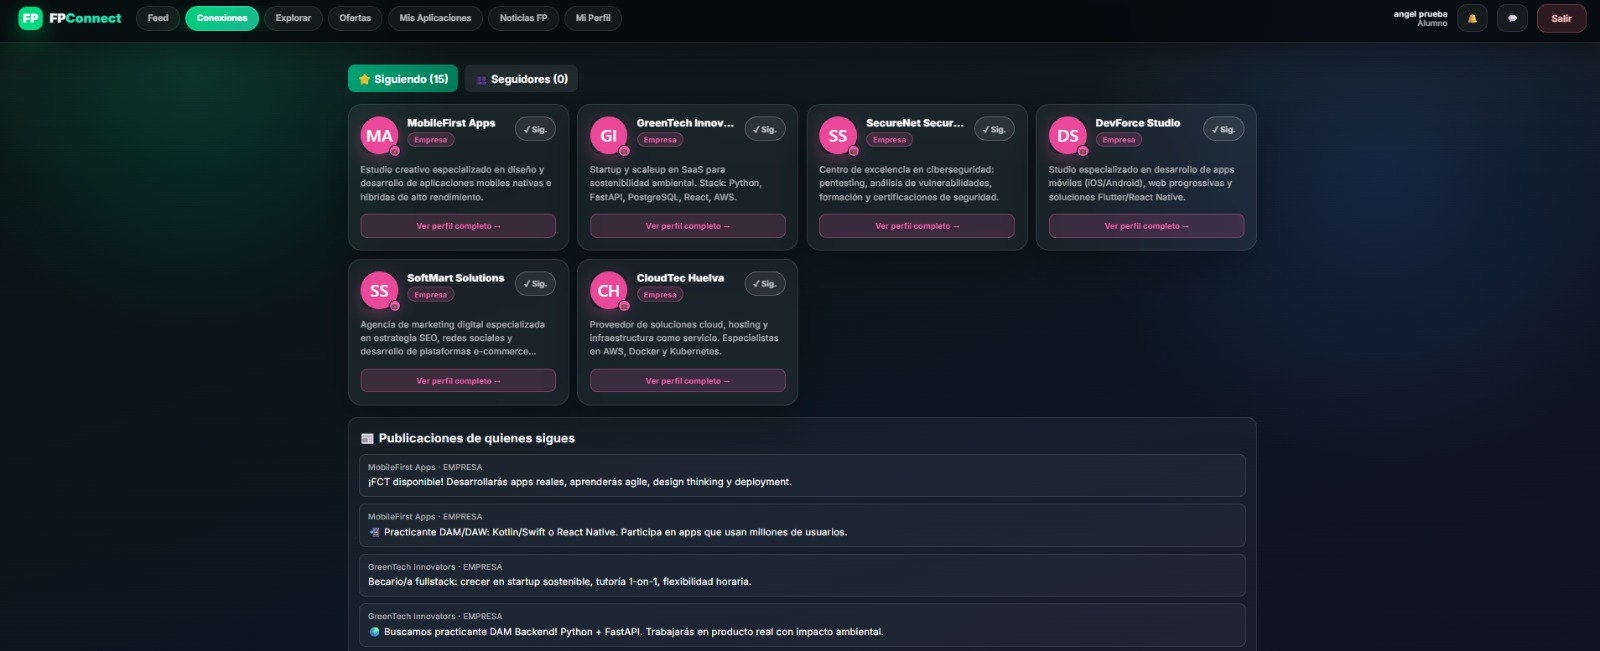
\includegraphics[width=0.75\textwidth]{images/01_login_page.jpg}
  \caption{Página de login: accede con tu cuenta o con Google}
  \label{fig:login_manual}
\end{figure}

\section{Recuperar contraseña}

Si olvidaste tu contraseña, haz clic en \textbf{``¿Olvidaste la contraseña?''} en la página de inicio de sesión. Recibirás instrucciones en tu correo electrónico para restablecerla.

\newpage

% ════════════════════════════════════════════════════════════════════════════
\chapter{Interfaz de Alumnos}
% ════════════════════════════════════════════════════════════════════════════

\section{Tu perfil de alumno}

Al acceder como alumno, verás un dashboard personalizado con múltiples secciones:

\subsection{Noticias FP}

La sección de \textbf{Noticias FP} te mantiene informado sobre:

\begin{itemize}
  \item Becas y ayudas para estudiantes de FP
  \item Convocatorias abiertas de selección
  \item Oportunidades de prácticas en empresas
  \item Noticias relevantes del sector de Formación Profesional
  \item Seminarios, webinars y eventos educativos
\end{itemize}

\begin{figure}[H]
  \centering
  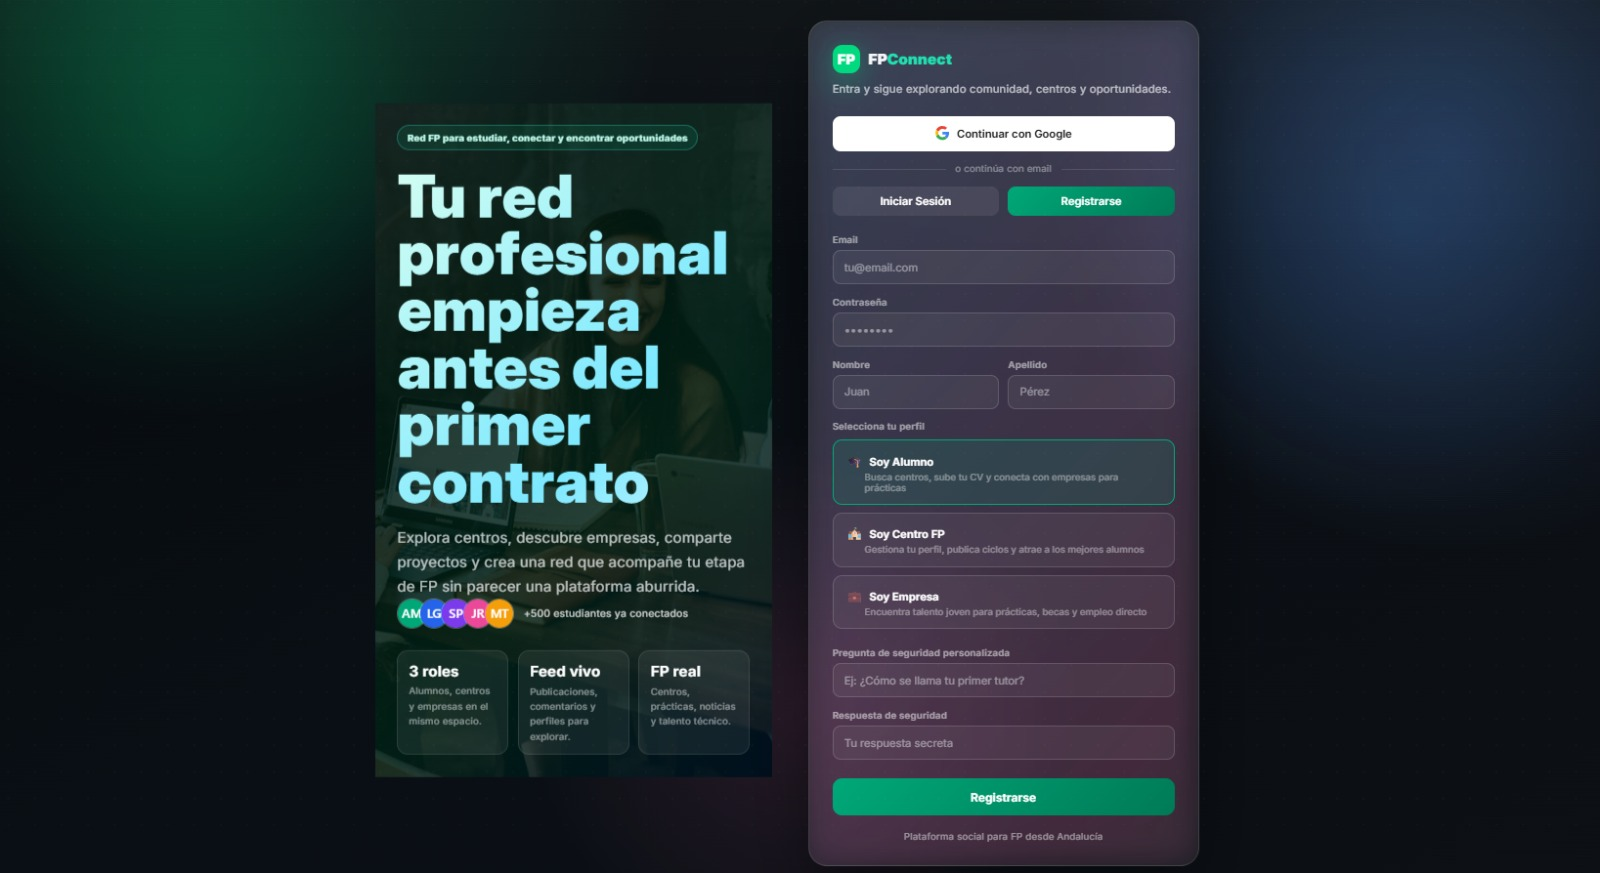
\includegraphics[width=0.8\textwidth]{images/03_noticias_fp.jpg}
  \caption{Sección de Noticias FP: mantente informado de becas y oportunidades}
  \label{fig:noticias_manual}
\end{figure}

\subsection{Feed de Actividad}

El \textbf{Feed} es el centro social de FPConnect. Aquí puedes:

\begin{itemize}
  \item \textbf{Crear publicaciones:} Comparte tus experiencias, consejos o proyectos con un clic en \textbf{``Comparte algo útil''}
  \item \textbf{Interactuar:} Dale like, comenta o comparte publicaciones de otros alumnos
  \item \textbf{Seguir usuarios:} Mantente actualizado de lo que publican tus contactos
  \item \textbf{Ver comentarios:} Haz clic en cualquier publicación para ver y añadir comentarios
\end{itemize}

\begin{figure}[H]
  \centering
  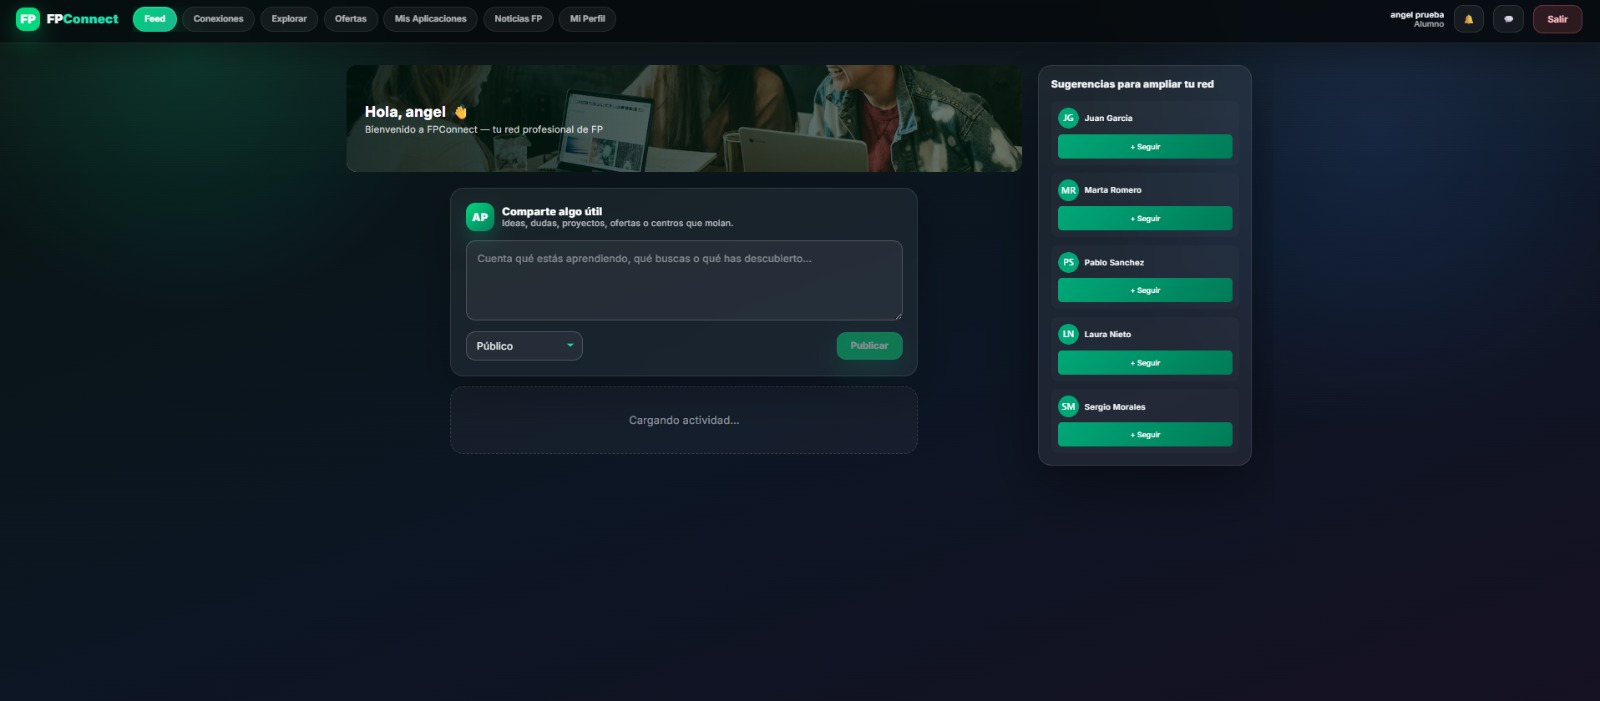
\includegraphics[width=0.8\textwidth]{images/04_feed_actividad.jpg}
  \caption{Feed de actividad: comparte publicaciones e interactúa con otros}
  \label{fig:feed_manual}
\end{figure}

\subsection{Explorador de Empresas}

Busca empresas colaboradoras filtradas por:

\begin{itemize}
  \item \textbf{Provincia:} Todas, Almería, Cádiz, Córdoba, etc.
  \item \textbf{Sector:} Tecnología, Construcción, Sanidad, Turismo, etc.
  \item \textbf{Especialidad:} Busca por especialidad profesional
\end{itemize}

Al encontrar una empresa que te interesa, puedes ver su perfil completo y solicitar conexión.

\begin{figure}[H]
  \centering
  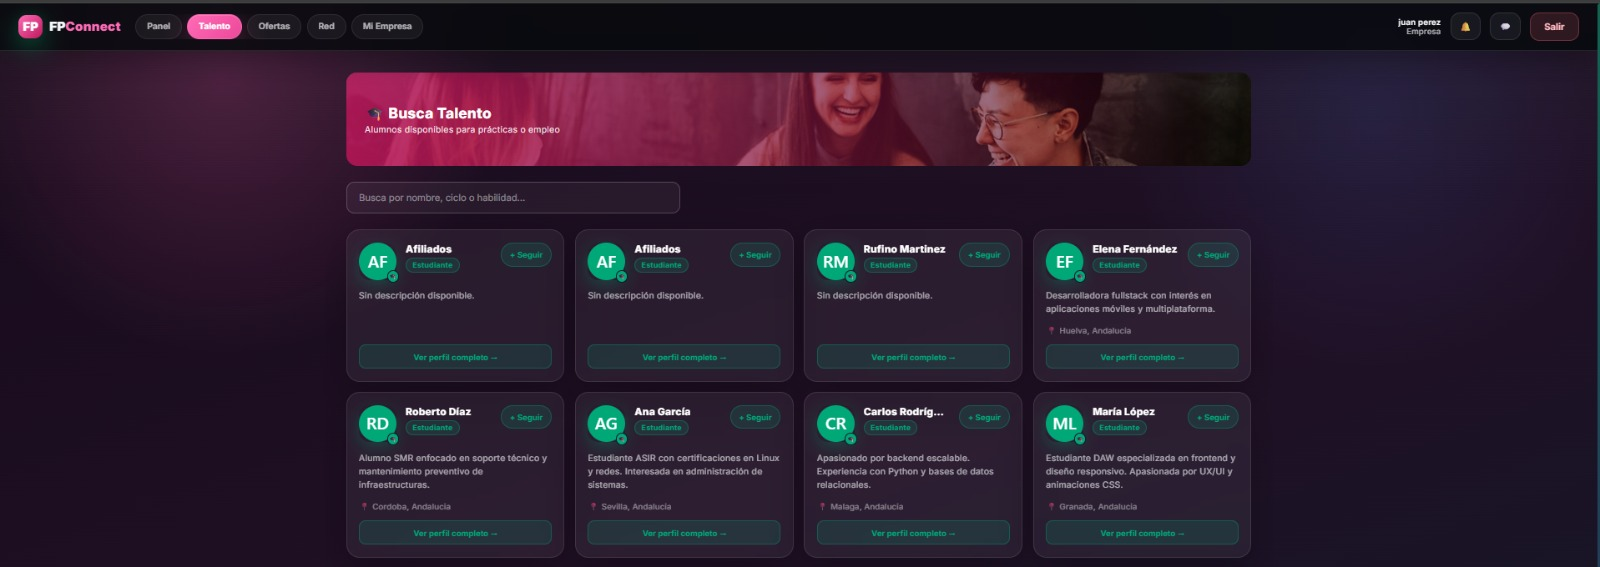
\includegraphics[width=0.8\textwidth]{images/05_explorador_empresas.jpg}
  \caption{Explorador de empresas: encuentra empresas colaboradoras}
  \label{fig:empresas_manual}
\end{figure}

\subsection{Buscar Talento}

Conecta con otros alumnos de tu ciclo o especialidad:

\begin{itemize}
  \item \textbf{Ciclo:} Filtra por Grado Medio o Superior
  \item \textbf{Especialidad:} Selecciona tu área de estudio
  \item \textbf{Ubicación:} Busca por provincia
\end{itemize}

Haz clic en el botón \textbf{``Seguir Alumno''} para conectar con otros compañeros.

\begin{figure}[H]
  \centering
  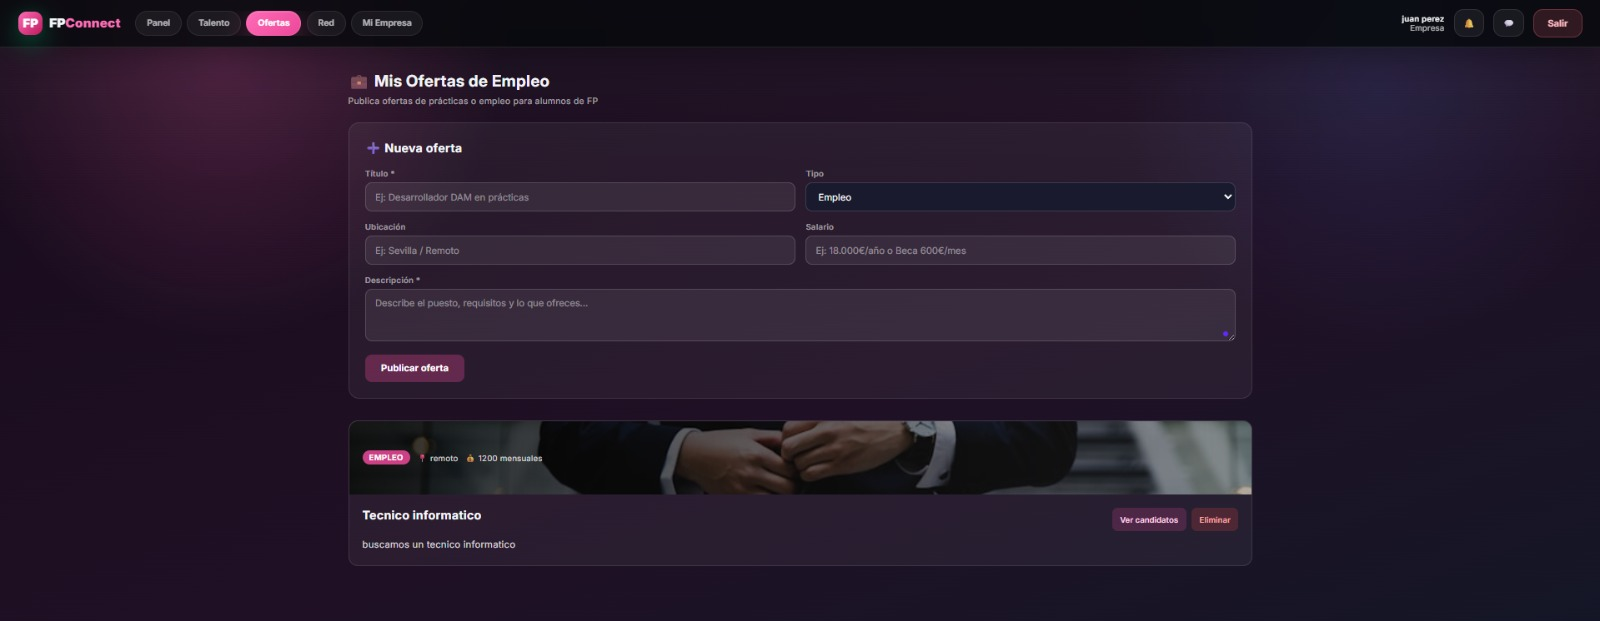
\includegraphics[width=0.8\textwidth]{images/06_buscar_talento.jpg}
  \caption{Búsqueda de talento: conecta con otros alumnos}
  \label{fig:talento_manual}
\end{figure}

\subsection{Mis Conexiones}

Gestiona tu red profesional:

\begin{itemize}
  \item \textbf{Solicitudes pendientes:} Revisa y acepta/rechaza solicitudes de conexión
  \item \textbf{Mis contactos:} Visualiza todos tus contactos aceptados
  \item \textbf{Seguidos:} Ve a quién estás siguiendo
\end{itemize}

\begin{figure}[H]
  \centering
  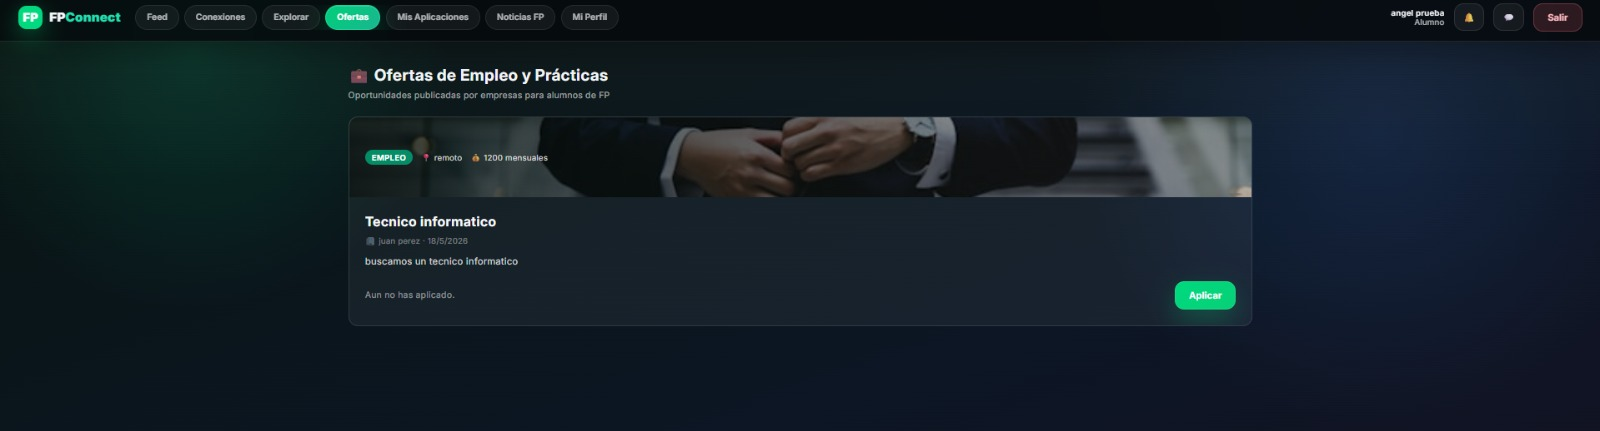
\includegraphics[width=0.8\textwidth]{images/07_conexiones_alumnos.jpg}
  \caption{Panel de conexiones: gestiona tu red de contactos}
  \label{fig:conexiones_manual}
\end{figure}

\subsection{Ofertas de Empleo y Prácticas}

Busca oportunidades de empleo o prácticas (FCT):

\begin{itemize}
  \item \textbf{Filtrar:} Por ubicación, tipo de oferta (empleo/prácticas), sector, etc.
  \item \textbf{Ver detalles:} Haz clic en cualquier oferta para ver toda la información
  \item \textbf{Candidatarse:} Pulsa \textbf{``Aplicar''} para enviar tu candidatura a la empresa
  \item \textbf{Ver candidatos:} Las empresas pueden ver quién se ha candidatado
\end{itemize}

\begin{figure}[H]
  \centering
  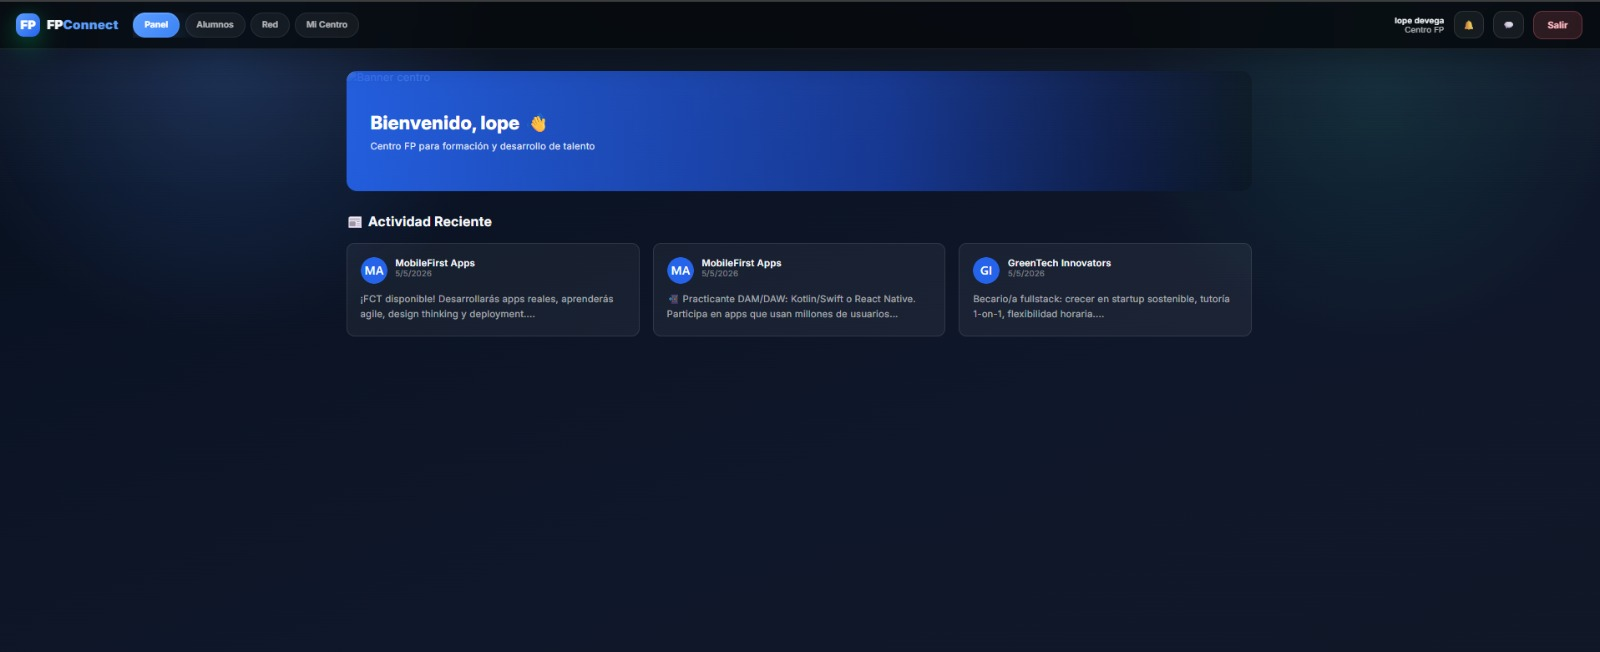
\includegraphics[width=0.8\textwidth]{images/08_ofertas_empleo.jpg}
  \caption{Ofertas de empleo y prácticas: encuentra oportunidades}
  \label{fig:ofertas_manual}
\end{figure}

\section{Mensajería en tiempo real}

Comunícate con otros usuarios sin esperas:

\begin{enumerate}
  \item Haz clic en el icono de \textbf{Mensajes} en la parte superior
  \item Selecciona un contacto existente o inicia una nueva conversación
  \item Escribe tu mensaje y presiona \textbf{Enviar}
  \item Los mensajes se entregan instantáneamente si el otro usuario está conectado
  \item Verás una notificación cuando recibas nuevos mensajes
\end{enumerate}

\section{Editar tu perfil}

Para actualizar tu información:

\begin{enumerate}
  \item Haz clic en tu avatar (esquina superior derecha)
  \item Selecciona \textbf{``Editar Perfil''}
  \item Actualiza tus datos:
  \begin{itemize}
    \item Avatar: Foto de perfil
    \item Biografía: Descripción breve sobre ti
    \item Ciclo: Tu ciclo formativo
    \item Especialidad: Tu especialidad
    \item Ubicación: Tu provincia
    \item Habilidades: Tus competencias técnicas
  \end{itemize}
  \item Haz clic en \textbf{``Guardar cambios''}
\end{enumerate}

\newpage

% ════════════════════════════════════════════════════════════════════════════
\chapter{Interfaz de Centros Educativos}
% ════════════════════════════════════════════════════════════════════════════

\section{Tu panel de centro}

Como centro educativo, accederás a un dashboard especializado:

\subsection{Alumnos Vinculados}

Gestiona los alumnos de tu centro:

\begin{itemize}
  \item \textbf{Ver lista:} Visualiza todos tus alumnos registrados en la plataforma
  \item \textbf{Buscar:} Filtra por nombre, ciclo o especialidad
  \item \textbf{Ver perfil:} Haz clic en cualquier alumno para ver su perfil completo
  \item \textbf{Comunicarse:} Envía mensajes a alumnos individuales
\end{itemize}

\begin{figure}[H]
  \centering
  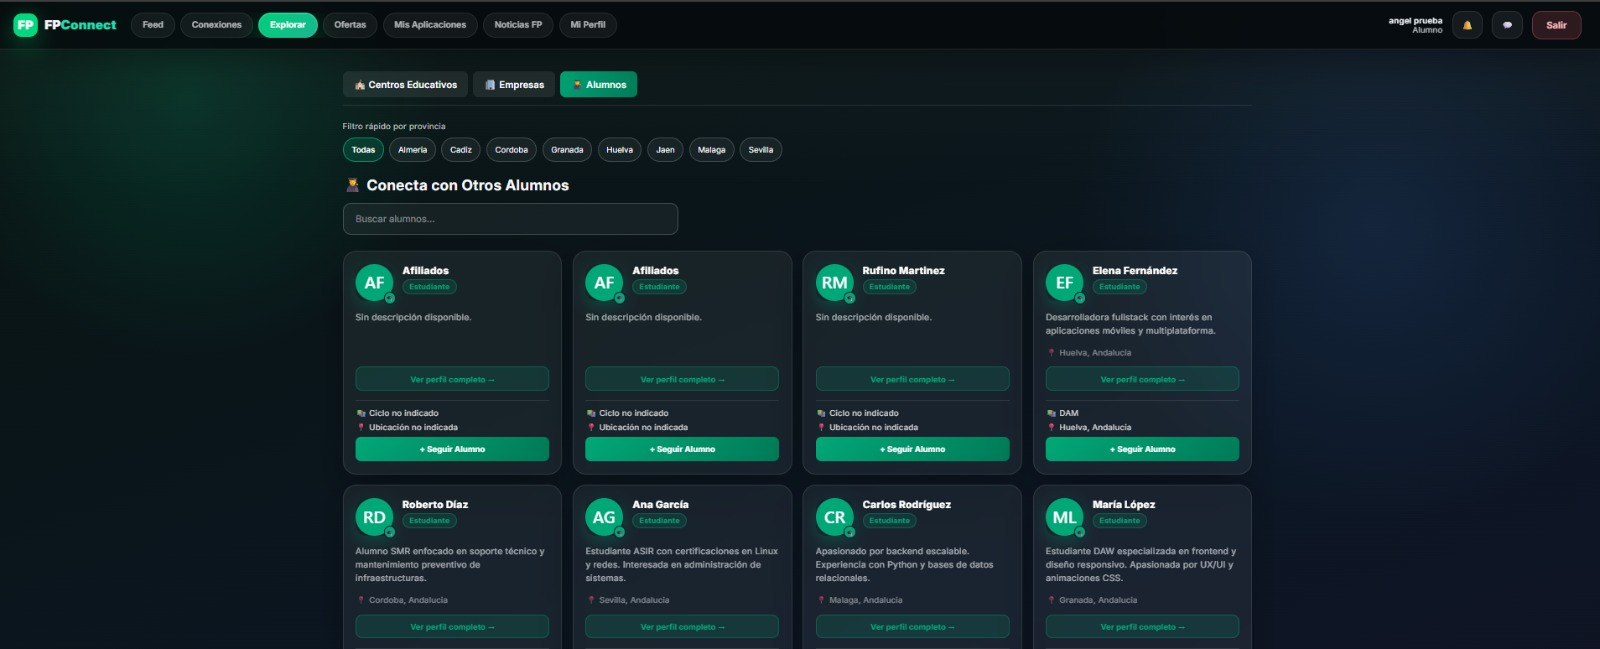
\includegraphics[width=0.8\textwidth]{images/12_alumnos_vinculados.jpg}
  \caption{Alumnos vinculados: gestiona los estudiantes de tu centro}
  \label{fig:alumnos_centro_manual}
\end{figure}

\subsection{Explorador de Centros}

Conecta con otros centros educativos:

\begin{itemize}
  \item \textbf{Buscar:} Por provincia, grado (Medio/Superior) o especialización
  \item \textbf{Ver detalles:} Información de contacto y ciclos ofertados
  \item \textbf{Solicitar conexión:} Para colaboraciones entre centros
\end{itemize}

\begin{figure}[H]
  \centering
  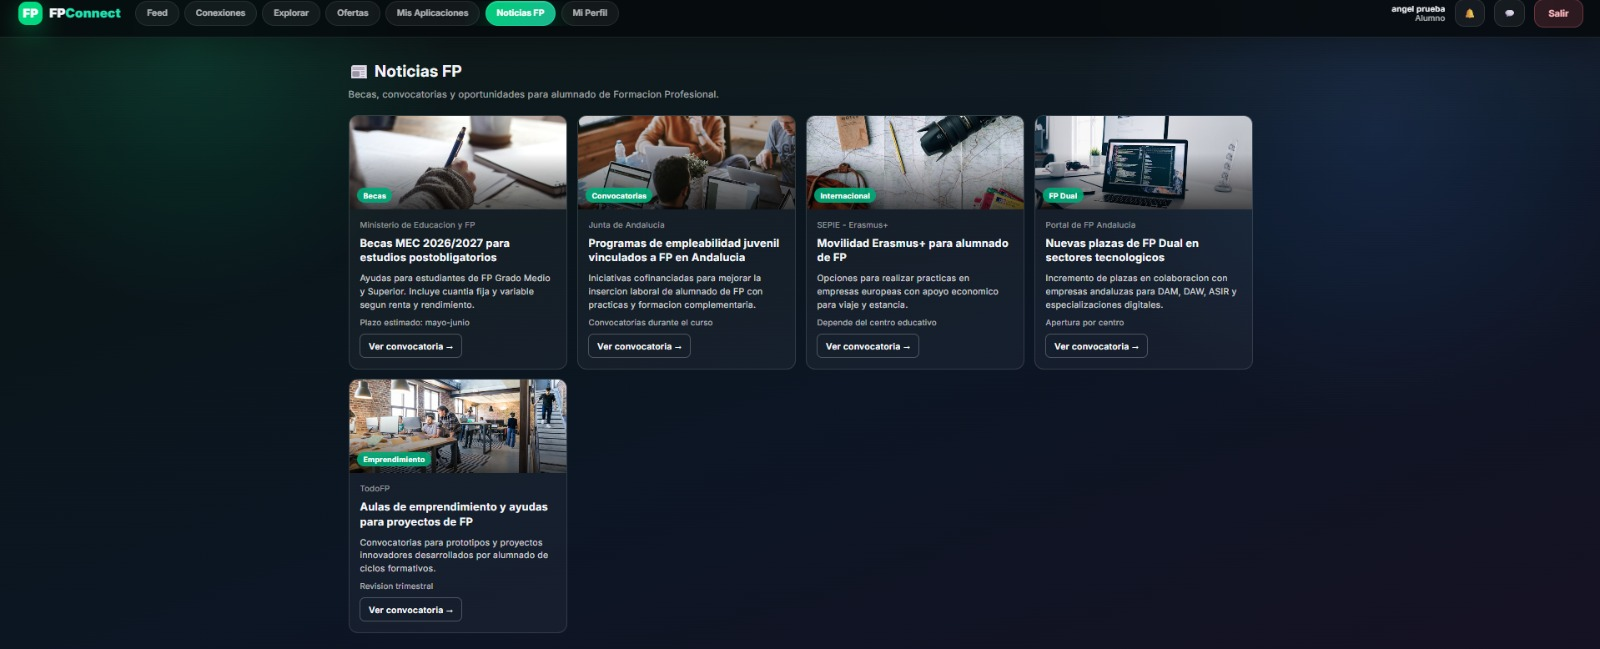
\includegraphics[width=0.8\textwidth]{images/13_explorador_centros.jpg}
  \caption{Explorador de centros: colabora con otros centros educativos}
  \label{fig:centros_explorer_manual}
\end{figure}

\subsection{Actividad Reciente}

Ve un resumen de:

\begin{itemize}
  \item Nuevos alumnos registrados desde tu centro
  \item Conexiones establecidas entre tus alumnos y empresas
  \item Publicaciones recientes de tu comunidad
  \item Ofertas de empleo para tus estudiantes
\end{itemize}

\begin{figure}[H]
  \centering
  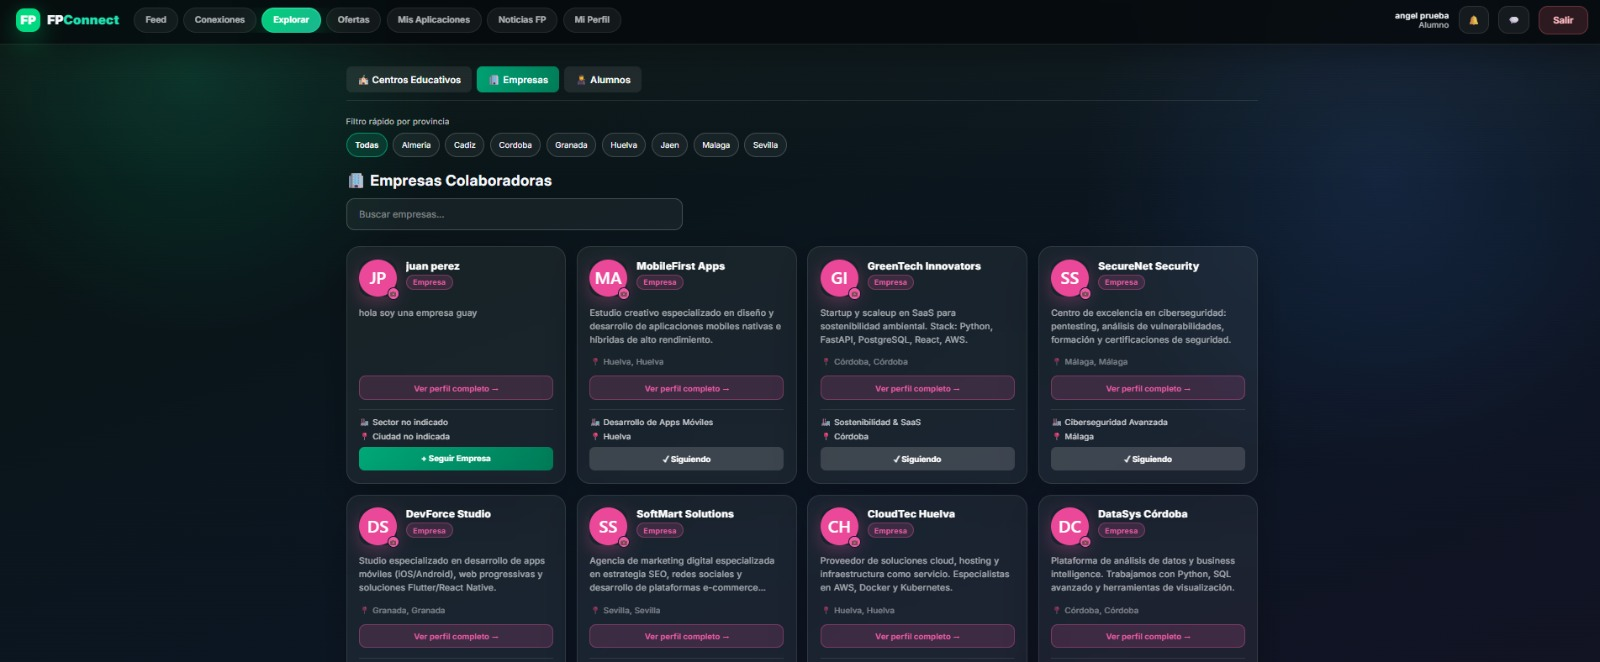
\includegraphics[width=0.8\textwidth]{images/11_centro_bienvenida.jpg}
  \caption{Bienvenida Centro FP: resumen de actividad}
  \label{fig:centro_bienvenida_manual}
\end{figure}

\section{Comunicación con empresas}

Establece relaciones con empresas colaboradoras:

\begin{enumerate}
  \item Busca empresas en el \textbf{Explorador}
  \item Solicita conexión para colaboraciones
  \item Una vez aceptada, envía mensajes directos
  \item Negocia plazas de prácticas (FCT) para tus alumnos
\end{enumerate}

\newpage

% ════════════════════════════════════════════════════════════════════════════
\chapter{Interfaz de Empresas}
% ════════════════════════════════════════════════════════════════════════════

\section{Tu dashboard de empresa}

Como empresa, tendrás acceso a funcionalidades especializadas:

\subsection{Búsqueda de Talento}

Encuentra candidatos cualificados:

\begin{itemize}
  \item \textbf{Filtrar:} Por ciclo, especialidad, ubicación, skills
  \item \textbf{Ver perfil:} Información completa del alumno
  \item \textbf{Conectar:} Envía solicitud de conexión
  \item \textbf{Mensaje directo:} Comunícate privadamente con candidatos
\end{itemize}

\begin{figure}[H]
  \centering
  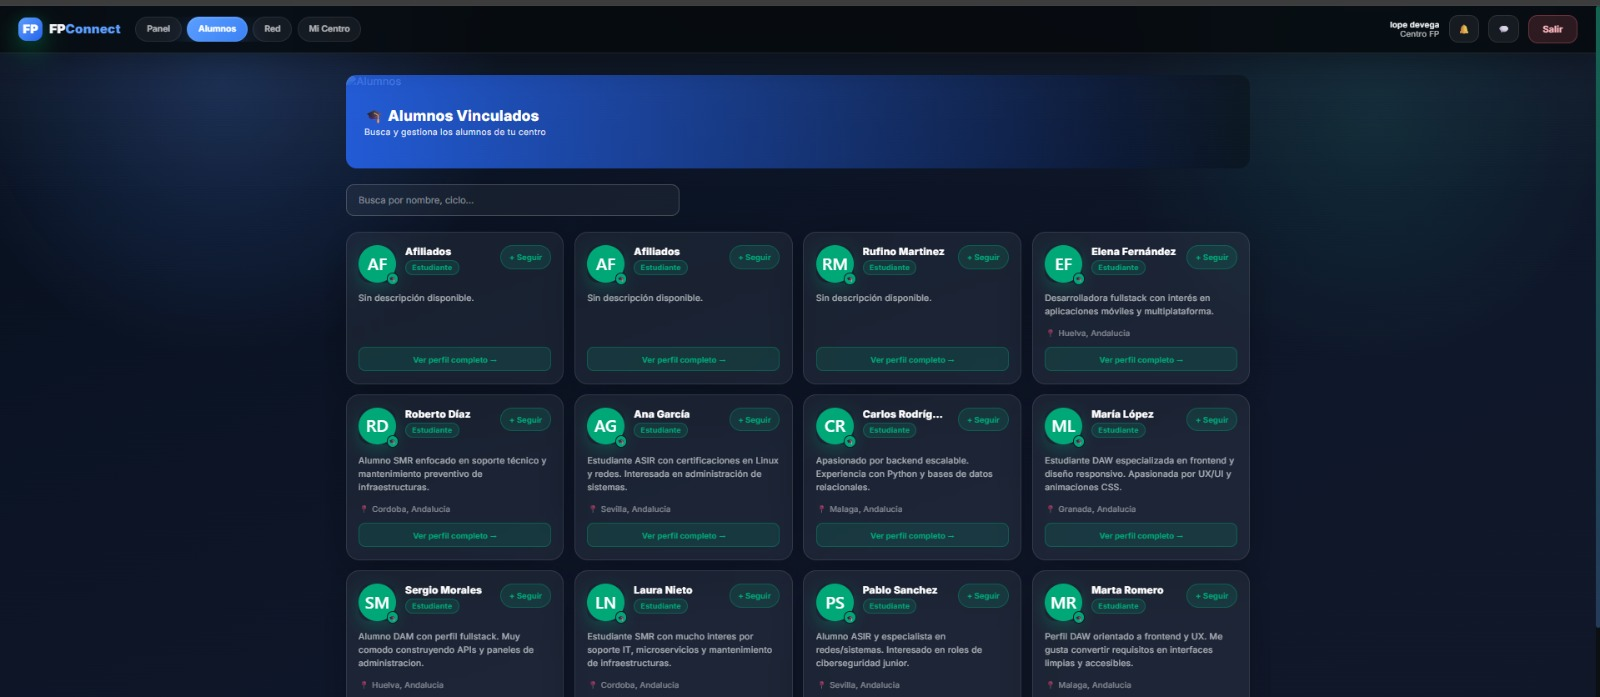
\includegraphics[width=0.8\textwidth]{images/09_empresa_bienvenida.jpg}
  \caption{Bienvenida Empresa: panel de gestión de candidatos}
  \label{fig:empresa_bienvenida_manual}
\end{figure}

\subsection{Crear Ofertas de Empleo}

Publica oportunidades para captar talento:

\begin{enumerate}
  \item Haz clic en \textbf{``Nueva Oferta''} en el panel
  \item Completa el formulario:
  \begin{itemize}
    \item \textbf{Título:} Nombre del puesto (ej: ``Técnico Informático'')
    \item \textbf{Tipo:} Elige entre Empleo o Prácticas (FCT)
    \item \textbf{Ubicación:} Provincia o ciudad donde se desarrollará el trabajo
    \item \textbf{Salario:} Rango salarial (opcional)
    \item \textbf{Descripción:} Detalla responsabilidades, requisitos, beneficios, etc.
  \end{itemize}
  \item Haz clic en \textbf{``Publicar oferta''}
  \item La oferta aparecerá inmediatamente en la plataforma
\end{enumerate}

\begin{figure}[H]
  \centering
  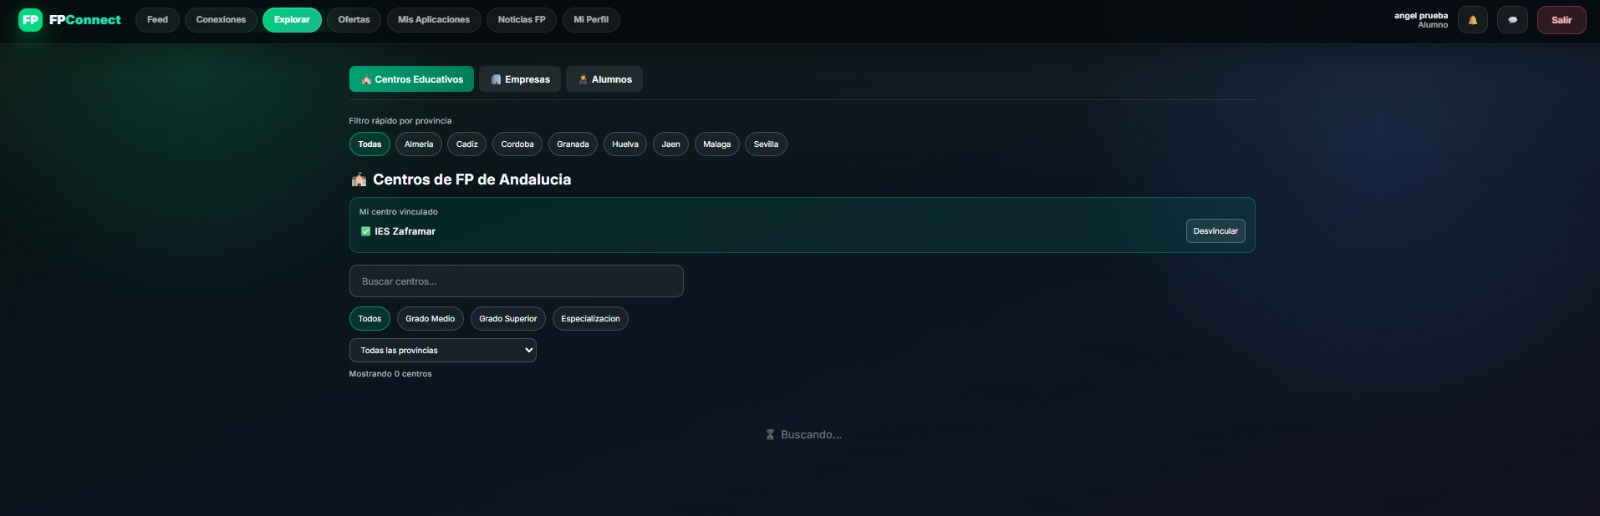
\includegraphics[width=0.8\textwidth]{images/10_empresa_crear_oferta.jpg}
  \caption{Crear oferta de empleo: publica oportunidades para candidatos}
  \label{fig:crear_oferta_manual}
\end{figure}

\subsection{Gestión de Candidaturas}

Revisa candidaturas a tus ofertas:

\begin{itemize}
  \item \textbf{Ver candidatos:} Haz clic en ``Ver candidatos'' en cada oferta
  \item \textbf{Revisar perfiles:} Examina el perfil completo de cada candidato
  \item \textbf{Contactar:} Envía mensajes privados a candidatos que te interesen
  \item \textbf{Eliminar oferta:} Cuando se cubra la plaza, elimina la oferta
\end{itemize}

\subsection{Conexiones Comerciales}

Construye relaciones B2B:

\begin{enumerate}
  \item \textbf{Buscar centros:} Usa el explorador de centros educativos
  \item \textbf{Conectar:} Solicita conexión para futuras colaboraciones
  \item \textbf{Negociar:} Acuerda plazas de prácticas (FCT) con centros
  \item \textbf{Comunicación:} Mantén conversaciones mediante mensajería privada
\end{enumerate}

\newpage

% ════════════════════════════════════════════════════════════════════════════
\chapter{Características Generales}
% ════════════════════════════════════════════════════════════════════════════

\section{Notificaciones}

Recibe alertas sobre:

\begin{itemize}
  \item Nuevas solicitudes de conexión
  \item Mensajes privados sin leer
  \item Respuestas a tus publicaciones
  \item Nuevas ofertas que coinciden con tu perfil (alumnos)
  \item Candidatos a tus ofertas (empresas)
  \item Noticias relevantes del sector FP
\end{itemize}

Haz clic en el icono de campana (\raisebox{-2pt}{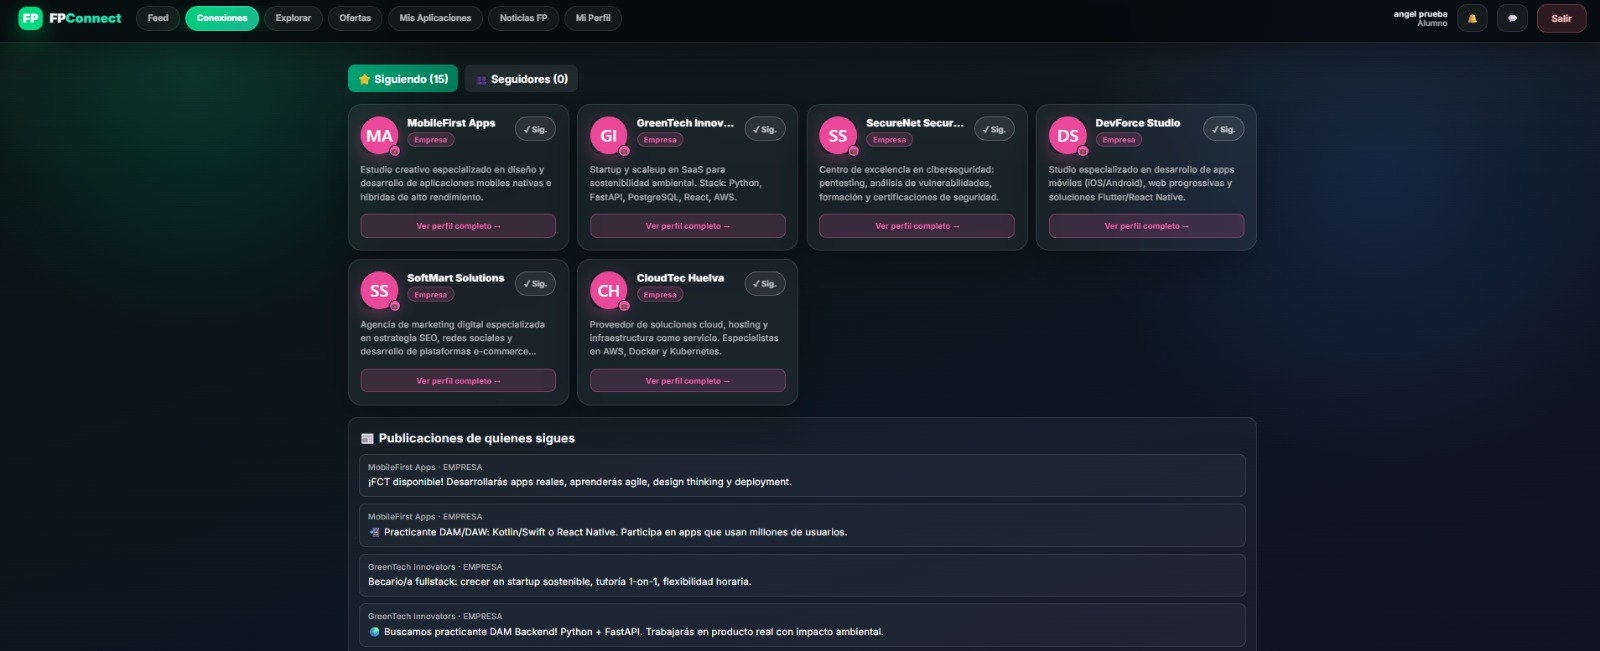
\includegraphics[width=0.3cm]{images/01_login_page.jpg}}) en la barra superior para ver todas tus notificaciones.

\section{Privacidad y Seguridad}

FPConnect protege tu información:

\begin{itemize}
  \item \textbf{Contraseña segura:} Usa contraseñas de al menos 8 caracteres
  \item \textbf{Verificación:} Confirma tu identidad mediante email
  \item \textbf{Tokens JWT:} Tu sesión está protegida con criptografía
  \item \textbf{HTTPS:} Toda la comunicación está encriptada
  \item \textbf{CORS protegido:} Solo tu navegador puede acceder a tus datos
\end{itemize}

\section{Configuración de Cuenta}

Personaliza tu experiencia:

\begin{enumerate}
  \item Haz clic en tu avatar (esquina superior derecha)
  \item Selecciona \textbf{``Configuración''}
  \item Opciones disponibles:
  \begin{itemize}
    \item Cambiar contraseña
    \item Privacidad de perfil
    \item Preferencias de notificaciones
    \item Tema oscuro/claro
    \item Idioma
  \end{itemize}
\end{enumerate}

\section{Cerrar Sesión}

Para salir de tu cuenta:

\begin{enumerate}
  \item Haz clic en tu avatar
  \item Selecciona \textbf{``Cerrar Sesión''}
  \item Se guardará tu estado y podrás volver a conectarte cuando quieras
\end{enumerate}

\newpage

% ════════════════════════════════════════════════════════════════════════════
\chapter{Preguntas Frecuentes (FAQ)}
% ════════════════════════════════════════════════════════════════════════════

\section{¿Cómo contacto con soporte?}

Si tienes problemas o sugerencias, contáctanos en:
\begin{itemize}
  \item \textbf{Email:} soporte@fpconnect.app
  \item \textbf{Web:} www.fpconnect.app/soporte
  \item \textbf{Redes sociales:} @fpconnect en Instagram y Twitter
\end{itemize}

\section{¿Mi contraseña es segura?}

Sí. Las contraseñas se almacenan con bcrypt, un algoritmo criptográfico especial que imposibilita recuperarlas incluso si alguien accede a los servidores.

\section{¿Puedo cambiar mi tipo de usuario?}

Por el momento, no. Deberás crear una nueva cuenta. En futuras versiones permitiremos cambiar de rol.

\section{¿Se puede publicar contenido desde móvil?}

Sí. FPConnect es responsive y funciona perfectamente en dispositivos móviles, tablets y computadoras de escritorio.

\section{¿Hay límite de conexiones?}

No, puedes conectar con tantos usuarios como desees.

\section{¿Cuáles son los horarios de disponibilidad?}

FPConnect está disponible 24/7. El mantenimiento preventivo se realiza los domingos de 2:00 a 3:00 AM.

\section{¿Cómo elimino mi cuenta?}

Contáctanos en soporte@fpconnect.app para solicitar la eliminación. Se eliminarán todos tus datos en 30 días.

\newpage

% ════════════════════════════════════════════════════════════════════════════
\chapter*{Conclusión}
\addcontentsline{toc}{chapter}{Conclusión}
% ════════════════════════════════════════════════════════════════════════════

Esperamos que este manual te haya ayudado a familiarizarte con FPConnect. La plataforma está en constante evolución, y estamos agregando nuevas funcionalidades regularmente basadas en el feedback de usuarios como tú.

Si tienes sugerencias o encuentras problemas, no dudes en contactarnos. Tu opinión es fundamental para mejorar la experiencia de toda la comunidad de Formación Profesional.

¡Que disfrutes usando FPConnect y te deseamos mucho éxito en tu carrera profesional!

\end{document}
